\section{Optimización}
La optimización es una herramienta que nos ayuda a encontrar \textit{la mejor} entre diferentes opciones elegibles. En nuestra vida diaria a menudo nos encontramos en este tipo de situaciones, por ejemplo al elegir entre diferentes rutas para llegar a algún lugar.

Formalmente, un problema de optimización consiste en hallar el mínimo o máximo de una función $f:X\rightarrow \mathbb{R}x$ (llamada función objetivo) en un conjunto de soluciones $X$. De modo que el problema consiste en hallar:
\begin{gather}
\min_{x\in X} f(x)
\end{gather}
Es importante mencionar que cualquier problema de maximización puede transformarse en un problema equivalente de minimiación con el reemplazo $f(x) \leftarrow -f(x)$, por lo que se considera solo el caso de minimización sin pérdida de generalidad.\\

Hallar el mínimo de la función sobre todo el conjunto $X$ recibe el nombre de optimización global, esto puede llegar a ser muy costoso o incluso imposible de obtener por lo que es común optar por obtener un mínimo local, es decir una solución que sea mejor que cualquiera de las soluciones que tiene a la misma distancia de acuerdo con alguna medida.
% mencionar optimimizacion continua, discreta
%\subsection*{Optimización continua vs}
\\ En la definición anterior no se requiere que el conjunto de soluciones tenga alguna propiedad o alguna estructura adicional. Por ejemplo el conjunto de soluciones puede ser un conjunto numerable ( i.e. los enteros ) o no numerable ( i.e. los números reales ). Estos dos casos dividen a la optimización en dos ramas: optimización continua y optimización discreta. En general los problemas de optimización suelen ser más fáciles de abordar\cite{nocedal2006numerical} porque en muchas ocasiones es posible obtener información del valor de la función objetivo de puntos cercanos a cierto punto conocido mientras que en los problemas discretos esto rara vez puede hacerse.\\

Dentro de los problemas de optimización discreta se distinguen los problemas de optimización combinatoria. Formalmente un problema de optimización discreta consta de los siguientes elementos\cite{Blum2003}:
\begin{itemize}
    \item Un conjunto de variables $Z={z_1,z_2,...,z_n}$
    \item Dominio para cada variable $D_1,D_2,...,D_n$
    \item Restricciones entre variables
\end{itemize}

En muchos problemas de optimización combinatoria el conjunto de soluciones no tiene alguna estructura adicional que ayude a buscar el mínimo de la función objetivo; es raro que exista un ordenamiento de las soluciones o una medida de distancia entre ellas que brinde propiedades a la función objetivo tales como continuidad o suavidad las cuales facilitarían la búsqueda del mínimo. Dicho de otro modo, no tenemos una forma eficiente de explorar el espacio de búsqueda. Ante estas limitaciones surgieron técnicas conocidas como metaheurísticas que buscan facilitar la resolución de estos problemas.

\section{Metaheurísticas}
Es muy común que en nuestra cotidianidad nos enfrentemos a problemas tan difíciles o para los que tengamos tan poco tiempo de decisión que no podamos hacer un análisis riguroso, en estos casos es muy común que utilicemos algún método (posiblemente basado en la experiencia) que nos permita hallar una solución aceptable, por ejemplo, es común que reemplacemos el problema por uno más simple que sí podemos responder y cuya respuesta está relacionada con nuestro problema original.\footnote{No podemos predecir con certeza si lloverá durante el día pero sí podemos responder si el cielo está plagado de nubes oscuras}  

En el contexto de la optimización una metaheurística es una metodología de alto nivel que combina diferentes heurísticas y puede aplicarse para resolver de manera aproximada una gran cantidad de problemas. En la práctica existen numerosas metaheuristicas que pueden ser muy diferentes entre sí por lo que no hay un sistema de clasificación universalmente aceptado aunque se han propuesto diferentes criterios de clasificación \cite{Stegherr2020} así como características como:
\begin{itemize}
\item De trayectoria vs discontinua. Una metaheurística de trayectoria consiste en, dada una solución inicial, mejorarla de manera iterativa mediante algún operador que <<mueve>> a la solución a través del espacio de búsqueda %extender.
\item basadas en población vs basadas en una sola solución. En las metaheurísticas basadas en población se mantiene un conjunto de soluciones candidatas.
\item basadas en búsqueda local vs constructivas. Como se explicará más adelante, en la búsqueda local, el proceso de mejora implica la evaluación de soluciones muy parecidas a una solución inicial dada mientras que en las constructivas se crean nuevas soluciones de acuerdo a una heurística o algoritmo preestablecido.
\item Con uso de memoria vs sin uso de memoria. El uso de memoria consiste en almacenar información que nos ayude a explorar el espacio de búsqueda, por ejemplo una lista de soluciones previamente visitadas.
\end{itemize} 
Los primeros dos de estos criterios están muy relacionados porque casi todas las metaheurísticas discontinuas son poblacionales y muchas de trayectoria son basadas en una sola solución.


Si bien las metaheurísticas son muy diversas existen elementos comunes que tienen un papel determinante en el buen funcionamiento de las mismas. En espécifico para las metaheurísticas de trayectoria existen tres conceptos que determinan cómo se ve el espacio de soluciones: las soluciones en sí, la forma en que las soluciones están conectadas y cómo podemos comparlas entre sí. A continuación se describebe cada uno de ellos
% introducir los conceptos siguientes
\subsection{Representación}
Puede ser que el problema de optimización en el que estemos interesados surja directamente de las matemáticas aunque si estamos interesados en un problema de nuestro entorno físico es necesario que tengamos una forma de traducirlo a un lenguaje matemático, incluidas las soluciones al mismo. Debemos encontrar una forma de representar de manera útil las soluciones posibles.
Por ejemplo si buscamos un ordenamiento óptimo para algún conjunto de $n$ cosas podemos asignarle a cada elemento del conjunto un número entero del $1$ al $n$, en este modelo el espacio de soluciones está constituido por todas las permutaciones de los números del $1$ al $n$. Hay varias maneras de representar permutaciones, podemos usar un arreglo de $n$ entradas o bien una matriz de permutación por mencionar algunos. Algo sumamente importante es que estas dos formas de representar las soluciones son muy distintas y se tiene que trabajar con ellas de manera muy diferente. La primera de ellas puede llegar a representar \textit{soluciones no factibles} por ejemplo que aparezca un número repetido, mientras que la segunda no.

Con el ejemplo anterior también podemos ver que cuando queramos establecer algunos operadores que, por ejemplo, perturben la solución tendremos que definirlos de maneras completamente distinta. Tambien es importante notar que es posible que las soluciones no factibles que podamos representar sean muchas más que las factibles.

Formalmente una represntación es un mapa que asocia elementos entre el conjunto de soluciones y el conjunto de las representaciones. Pueden distinguirse tres tipos de representaciones\cite{Cheng1996} de acuerdo a como asocian los elementos de estos dos conjuntos.
\begin{itemize}
    \item $1$ a $1$
    \item $1$ a $n$
    \item $n$ a $1$
\end{itemize}

% imagen de mapeo
\begin{figure}[H]
    \centering
    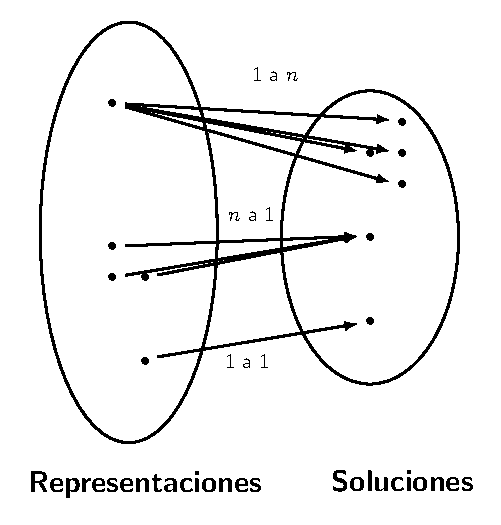
\includegraphics[scale=1]{Imagenes/representacion.pdf}
    \caption{Tipos de representaciones}
\end{figure}
Lo más conveniente suele ser un mapeo $1$ a $1$ y lo menos deseable es tener un mapeo $n$ a $1$.

\subsection{Vecindad}
La definicion de vecindad es crucial para las metaheurísticas de trayectoria y las basadas en una sola solución.
Formalmente, una vecindad es un mapeo $N:X\leftarrow 2^X$ que le asigna a cada solución $x\in X$ un subconjunto de soluciones en $X$. Intuitivamente podemos pensar que es una forma de definir a las soluciones que <<rodean>> a otra. Se dice que la solución $y$ es un vecino de $x$ si $y\in N(x)$.

A partir de la definición de vecindad podemos también definir un operador de movimiento cuyo efecto al aplicarlo a una solución sea transformarla en una que pertenezca a su vecindad, i.e. este operador selecciona a un vecino de la solución inicial.  
 
\subsection{Función de aptitud o fitness}
Aunque para un problema de optimización ya se tiene definida una función objetivo que se quiere minimizar, no siempre tenderemos el mejor desempeño de las metaheurísticas con solo esta función por lo que resulta benéfico plantear una nueva función a minimizar con la que tengamos mejor desempeño. Por ejemplo puede suceder que aunque dos soluciones tengan asociado el mismo valor de la función objetivo una de ellas posee características que la hacen un mejor punto de partida para alguna metaheuristica.

Esta función debe asociar a cada solución un elemento de un conjunto donde esté definido un ordenamiento total. En esencia esta función define un operador de comparación entre soluciones de modo que podemos elegir la mejor de dos soluciones.
\subsection{Paisaje de búsqueda}
Una vez que tenemos el espacio de búsqueda y operadores de cambio para generar nuevas soluciones a partir de otras, se define el espacio de búsqueda como un grafo dirigido en el que los nodos son las soluciones al problema y una solución $x$ está conectada a otra $y$ si podemos generar a $y$ aplicando los operadores de cambio a $x$.

Podemos asociar a cada solución en el espacio un valor de aptitud o fitness que mide la calidad de dicha solución. La adición de esta función de aptitud al espacio de búsqueda genera al paisaje de búsqueda.\\

\begin{figure}[H]
\centering
\subfigure[Soluciones]{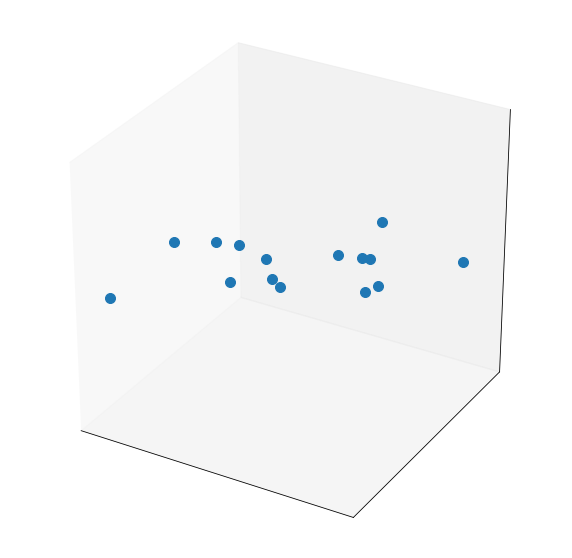
\includegraphics[scale=.4]{Imagenes/search1.png}}
\subfigure[Relaciones inducidas por los operadores de cambio]{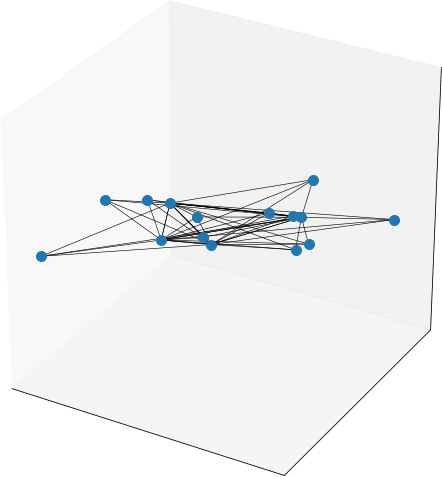
\includegraphics[scale=.4]{Imagenes/search2.png}}
\subfigure[Adición de la función de fitness]{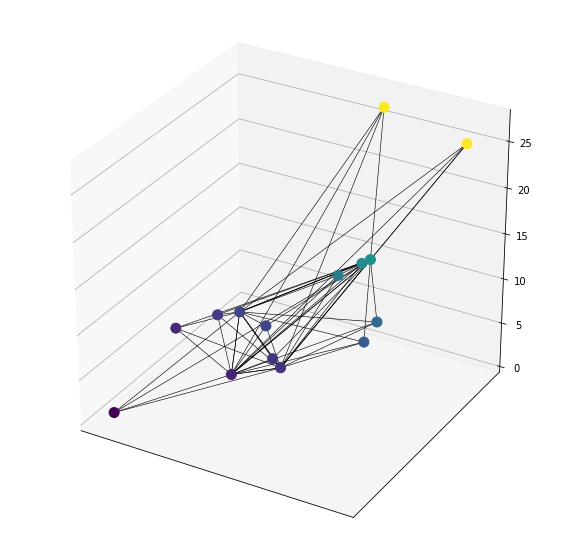
\includegraphics[scale=.4]{Imagenes/search3.png}}
\caption{Creación del paisaje de búsqueda}
\end{figure}

El paisaje de búsqueda es el <<terreno>> a explorar y puede cambiar si cambiamos cualquiera de sus componentes, podría ser que alguna representación nos centre en un subconjunto de soluciones convenientes o que alguna estructura de vecindad se proponga de modo que las mejores soluciones nunca estan muy lejos del resto, o que la función de fitness nos ayude a atravesar cúmulos de soluciones que serían iguales sin ella. Las metaheurísticas sirven como una estrategía para explorar el paisaje de búsqueda. Una de las más sencillas e intuitivas es conocida como escalada estocástica y simplemente consiste en reemplazar la solución actual por algún vecino mejor escogido al azar hasta que la solución en la que estemos sea mejor que todos sus vecinos, es decir, un ótimo local. Esta es una metaheurística de trayectoria y traza un camino entre las soluciones inicial y final.

%
%\begin{algorithm}[H]
% \KwData{Problema de Optimización}
%    \KwResult{Óptimo local $x$}
% Generar solución inicial $x$\;
% \doWhile{$L$ no vacía}{
%    Generar lista de vecinos $L$ de $x$\;
%    Escoger al azar un vecino $y\in L$\;
%  \eIf{y<x}{
%      x $leftarrow$ y\;
%      Generar lista de vecinos $L$ de $x$\;
%   }{
%       Quitar a $y$ de $L$\;
%  }
% }
%    \caption{Algoritmo de escalada estocástica}
%\end{algorithm}


\begin{figure}[H]
\centering
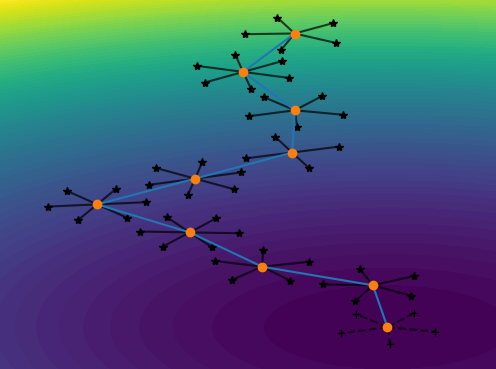
\includegraphics[scale=.5]{Imagenes/mettray.png}
    \caption{Ilustración de una escalada estocástica.\\ En cada paso se selecciona un vecino mejor que la solución actual hasta que la solución actual sea mejor que todos sus vecinos}
\end{figure}
% introducir ejemplos de mh de trayectoria

